\section{Risultati}\label{risultati}

\subsection{Tabella dei risultati}
\begin{center}
	\begin{tabular}{|c|c|c|c|c|c|}
		\hline
		\parbox{2cm}{\centering Istanza} & {Soluzione} & {Tempo(s)} & \parbox{2.75cm}{\vspace{.1cm}\centering Tempo Full Contraction(s)\vspace{.1cm}} & \parbox{2cm}{\centering Discovery time(s)} & {Errore(\%)}\\\hline
		input\_1\_6.txt & 2 & 0.00231 & 0.00007 & 0.00024 & 0.00\\\hline
		input\_2\_6.txt & 1 & 0.00174 & 0.00005 & 0.00065 & 0.00\\\hline
		input\_3\_6.txt & 3 & 0.00180 & 0.00006 & 0.00018 & 0.00\\\hline
		input\_4\_6.txt & 4 & 0.00217 & 0.00007 & 0.00014 & 0.00\\\hline
		input\_5\_10.txt & 4 & 0.03442 & 0.00030 & 0.00072 & 0.00\\\hline
		input\_6\_10.txt & 3 & 0.01447 & 0.00013 & 0.00095 & 0.00\\\hline
		input\_7\_10.txt & 2 & 0.01540 & 0.00013 & 0.00062 & 0.00\\\hline
		input\_8\_10.txt & 1 & 0.01490 & 0.00013 & 0.00013 & 0.00\\\hline
		input\_9\_25.txt & 7 & 1.59042 & 0.00158 & 0.00887 & 0.00\\\hline
		input\_10\_25.txt & 6 & 1.56295 & 0.00155 & 0.04115 & 0.00\\\hline
		input\_11\_25.txt & 8 & 2.00112 & 0.00199 & 0.00893 & 0.00\\\hline
		input\_12\_25.txt & 9 & 1.89574 & 0.00188 & 0.00201 & 0.00\\\hline
		input\_13\_50.txt & 15 & 60.00233 & 0.01549 & 0.10327 & 0.00\\\hline
		input\_14\_50.txt & 16 & 60.01616 & 0.01579 & 0.13614 & 0.00\\\hline
		input\_15\_50.txt & 14 & 60.00795 & 0.01347 & 0.04197 & 0.00\\\hline
		input\_16\_50.txt & 10 & 60.01186 & 0.01411 & 0.02720 & 0.00\\\hline
		input\_17\_75.txt & 19 & 60.01799 & 0.04756 & 0.12836 & 0.00\\\hline
		input\_18\_75.txt & 15 & 60.04845 & 0.05328 & 0.15721 & 0.00\\\hline
		input\_19\_75.txt & 18 & 60.03456 & 0.05216 & 0.40870 & 0.00\\\hline
		input\_20\_75.txt & 16 & 60.01651 & 0.05090 & 1.61908 & 0.00\\\hline
		input\_21\_100.txt & 22 & 60.11853 & 0.12656 & 0.74940 & 0.00\\\hline
		input\_22\_100.txt & 23 & 60.05595 & 0.12670 & 0.87588 & 0.00\\\hline
		input\_23\_100.txt & 19 & 60.05745 & 0.13680 & 0.56977 & 0.00\\\hline
		input\_24\_100.txt & 24 & 60.05831 & 0.13228 & 0.61221 & 0.00\\\hline
		input\_25\_125.txt & 34 & 60.23190 & 0.30267 & 2.83151 & 0.00\\\hline
		input\_26\_125.txt & 29 & 60.13841 & 0.27212 & 4.71717 & 0.00\\\hline
		input\_27\_125.txt & 36 & 60.06676 & 0.30336 & 0.91342 & 0.00\\\hline
		input\_28\_125.txt & 31 & 60.10401 & 0.25576 & 7.58857 & 0.00\\\hline
		input\_29\_150.txt & 37 & 60.17212 & 0.60780 & 3.03944 & 0.00\\\hline
		input\_30\_150.txt & 35 & 60.26632 & 0.52405 & 0.59696 & 0.00\\\hline
		input\_31\_150.txt & 41 & 60.51738 & 0.54033 & 2.94316 & 0.00\\\hline
		input\_32\_150.txt & 39 & 60.21118 & 0.56803 & 26.88796 & 0.00\\\hline
		input\_33\_175.txt & 42 & 60.69174 & 0.90584 & 2.62535 & 0.00\\\hline
		input\_34\_175.txt & 45 & 60.81718 & 0.90772 & 45.62800 & 0.00\\\hline
		input\_35\_175.txt & 53 & 60.90280 & 1.14911 & 10.99047 & 0.00\\\hline
		input\_36\_175.txt & 43 & 60.37577 & 0.86251 & 8.02117 & 0.00\\\hline
	\end{tabular}
\end{center}

\pagebreak

\begin{center}
	\begin{tabular}{|c|c|c|c|c|c|}
		\hline
		\parbox{2cm}{\centering Istanza} & {Soluzione} & {Tempo(s)} & \parbox{2.75cm}{\vspace{.1cm}\centering Tempo Full Contraction(s)\vspace{.1cm}} & \parbox{2cm}{\centering Discovery time(s)} & {Errore(\%)}\\\hline
		input\_37\_200.txt & 54 & 60.65795 & 1.68494 & 28.33442 & 0.00\\\hline
		input\_38\_200.txt & 52 & 61.38803 & 1.42763 & 18.03374 & 0.00\\\hline
		input\_39\_200.txt & 51 & 60.17441 & 1.50436 & 7.57775 & 0.00\\\hline
		input\_40\_200.txt & 61 & 61.56819 & 1.81083 & 12.76823 & 0.00\\\hline
	\end{tabular}
\end{center}

\subsection{Grafico di confronto dei tempi di esecuzione}
\begin{center}
	\begin{figure}[H]
		\centering
		\hspace{-1cm}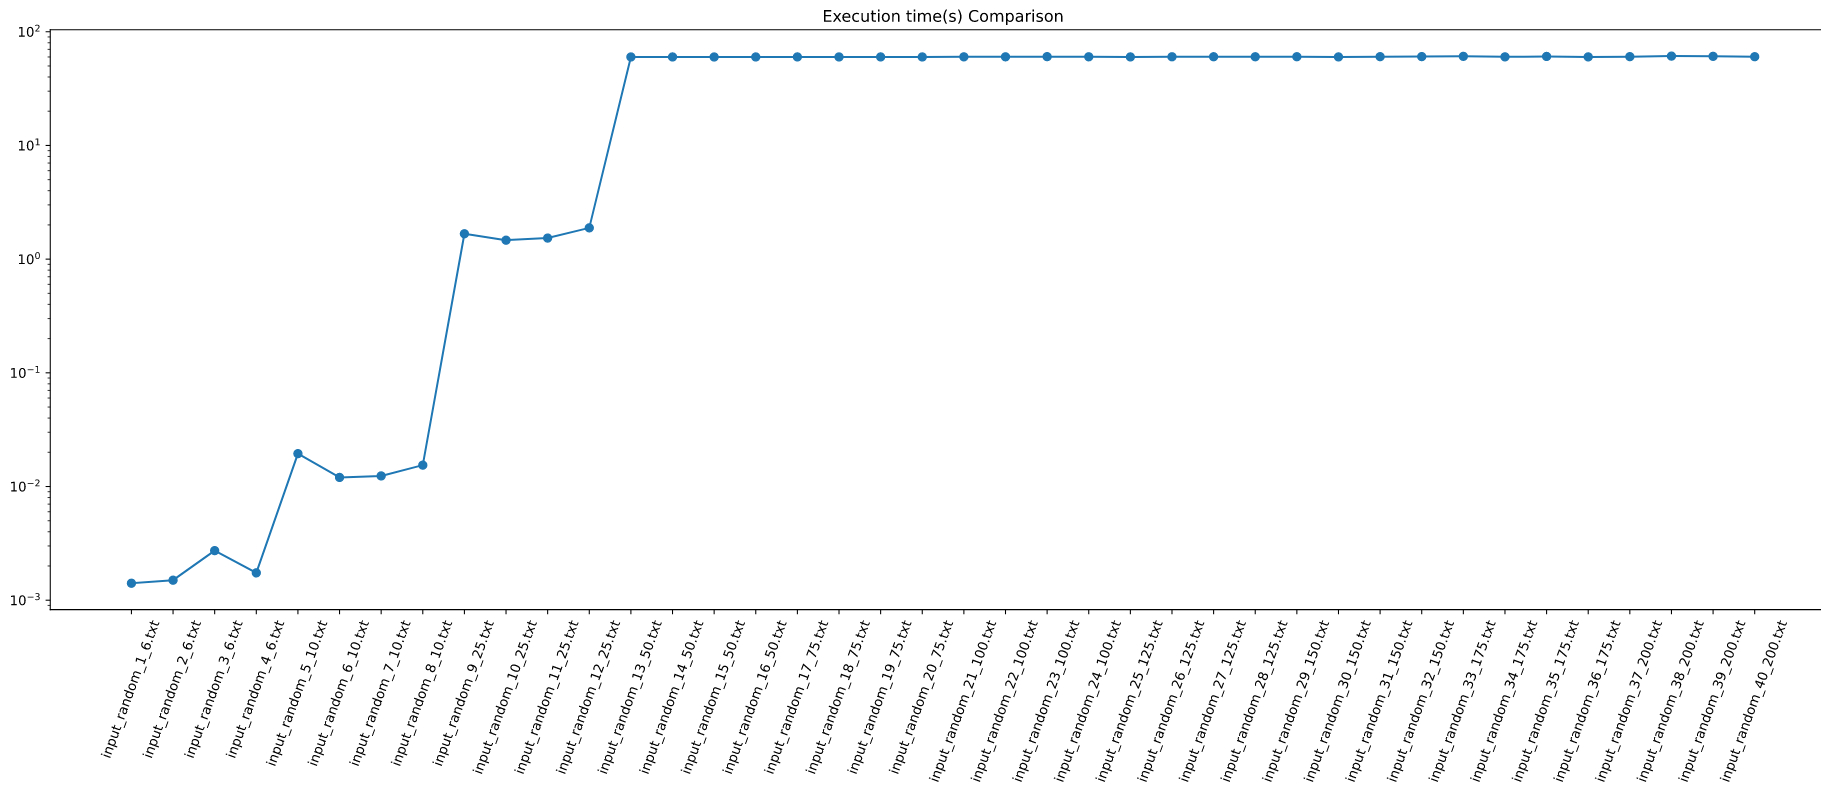
\includegraphics[width=\linewidth]{Img/exec_time_graph.jpg}
		\caption{Confronto dei tempi di esecuzione}
	\end{figure}
\end{center}

\subsection{Grafico di confronto dei tempi di Full Contraction}
\begin{center}\label{fc_time}
	\begin{figure}[H]
		\centering
		\hspace{-1cm}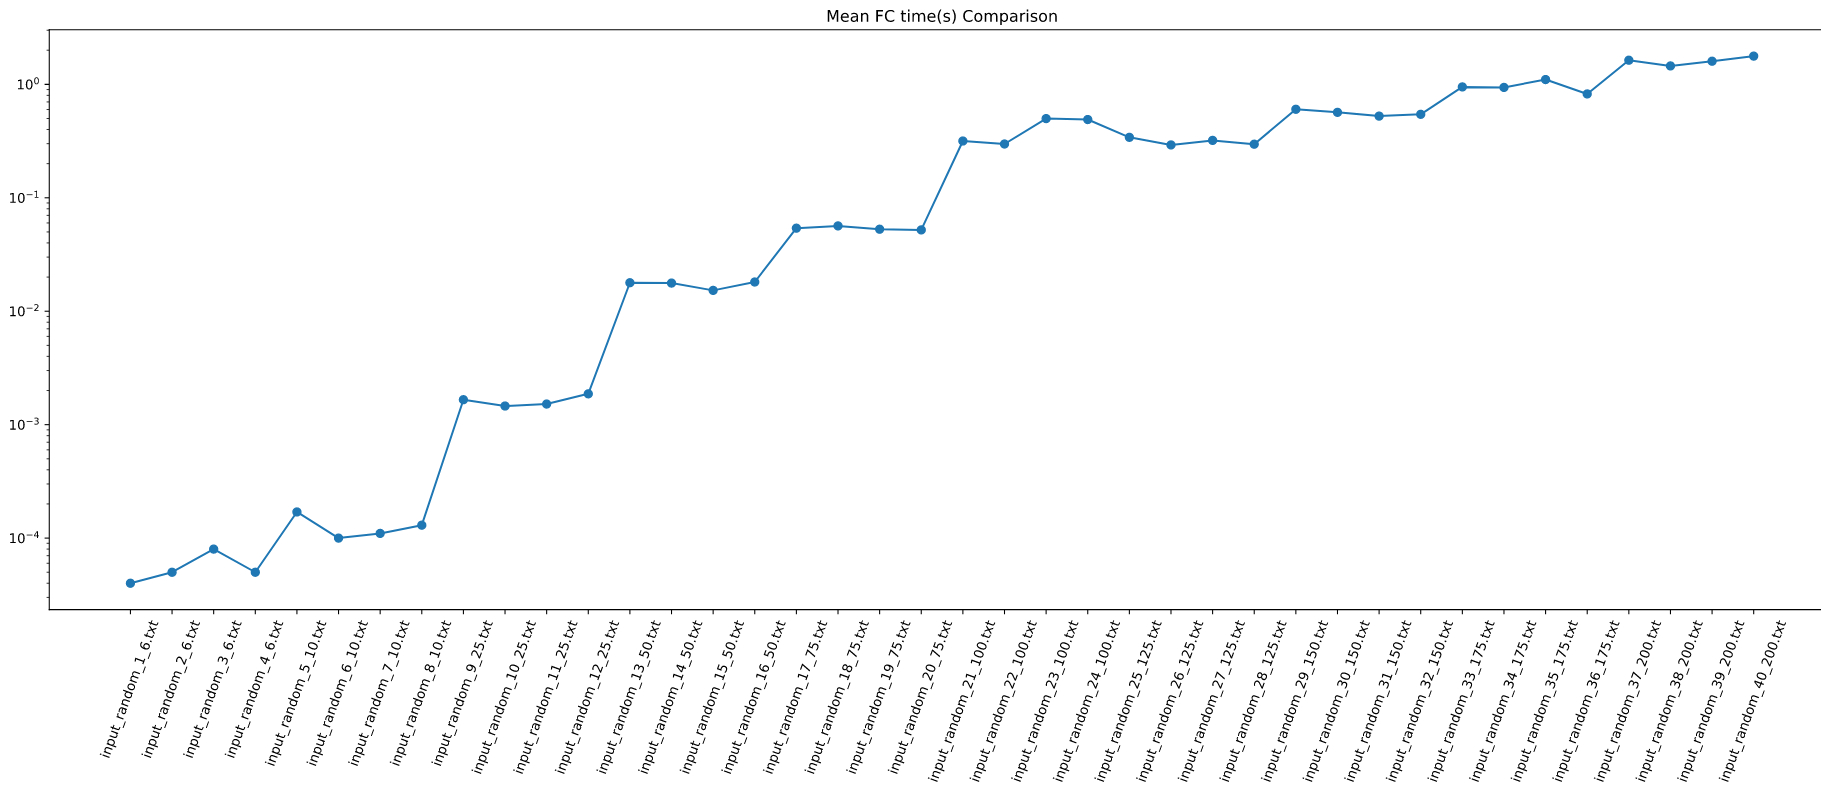
\includegraphics[width=\linewidth]{Img/fc_time_graph.jpg}
		\caption{Confronto dei tempi di Full Contraption}
	\end{figure}
\end{center}

\subsection{Grafico di confronto dei Discovery Time}
\begin{center}
	\begin{figure}[H]
		\centering
		\hspace{-1cm}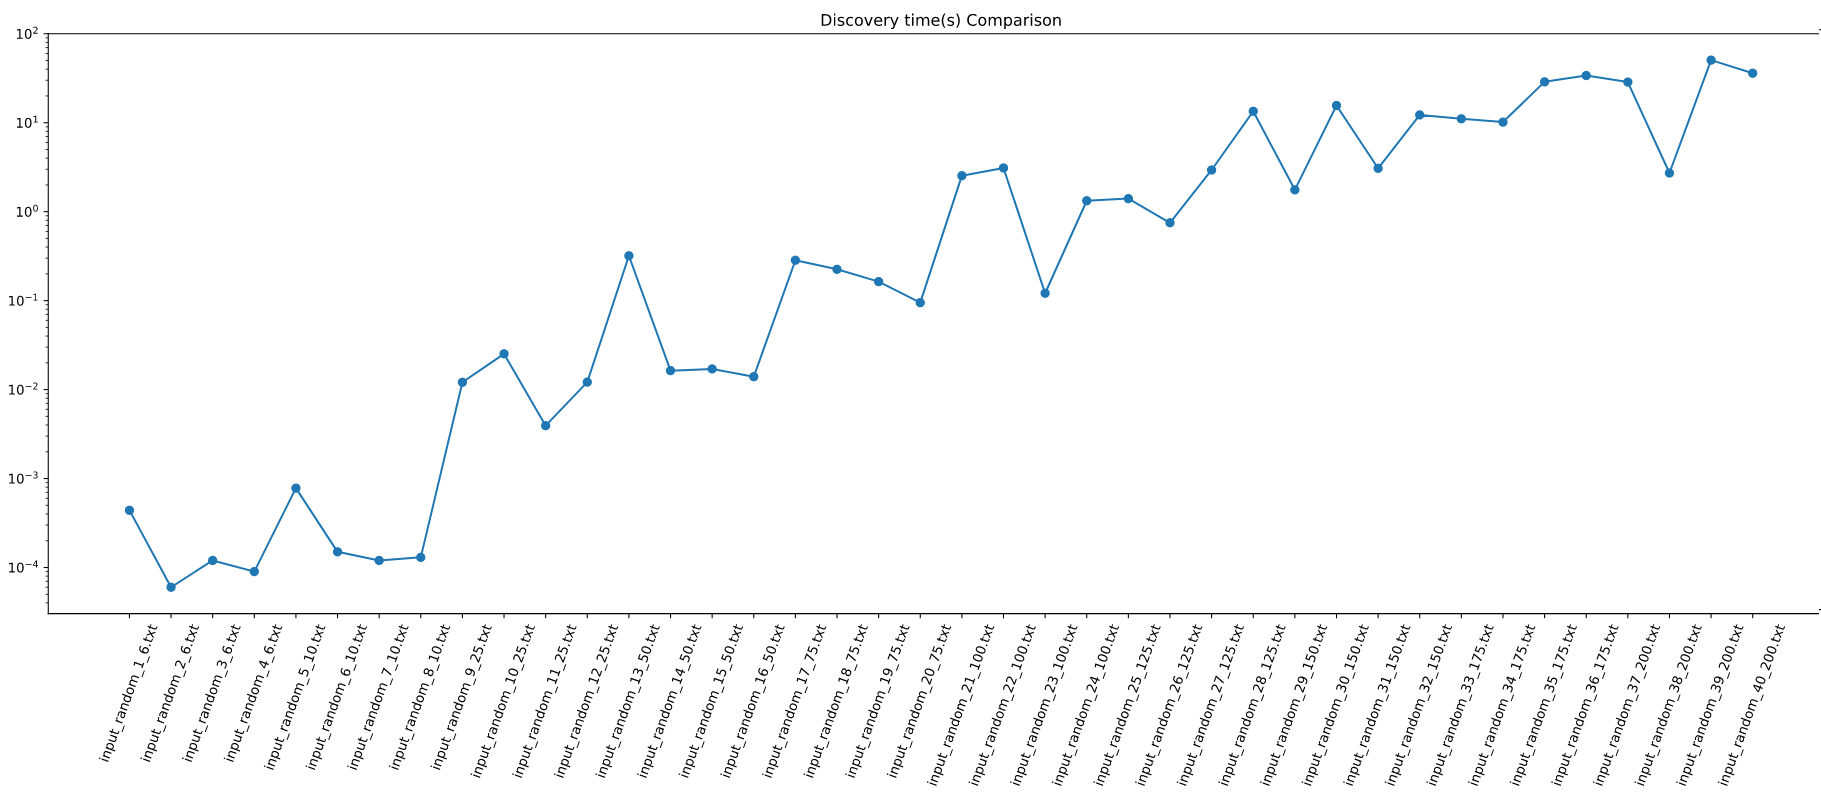
\includegraphics[width=\linewidth]{Img/disc_time_graph.jpg}
		\caption{Confronto dei Discovery Time}
	\end{figure}
\end{center}

\subsection{Grafico di confronto dei Discovery Time rispetto ai tempi totali}\label{confronto}
\begin{center}
	\begin{figure}[H]
		\centering
		\hspace{-1cm}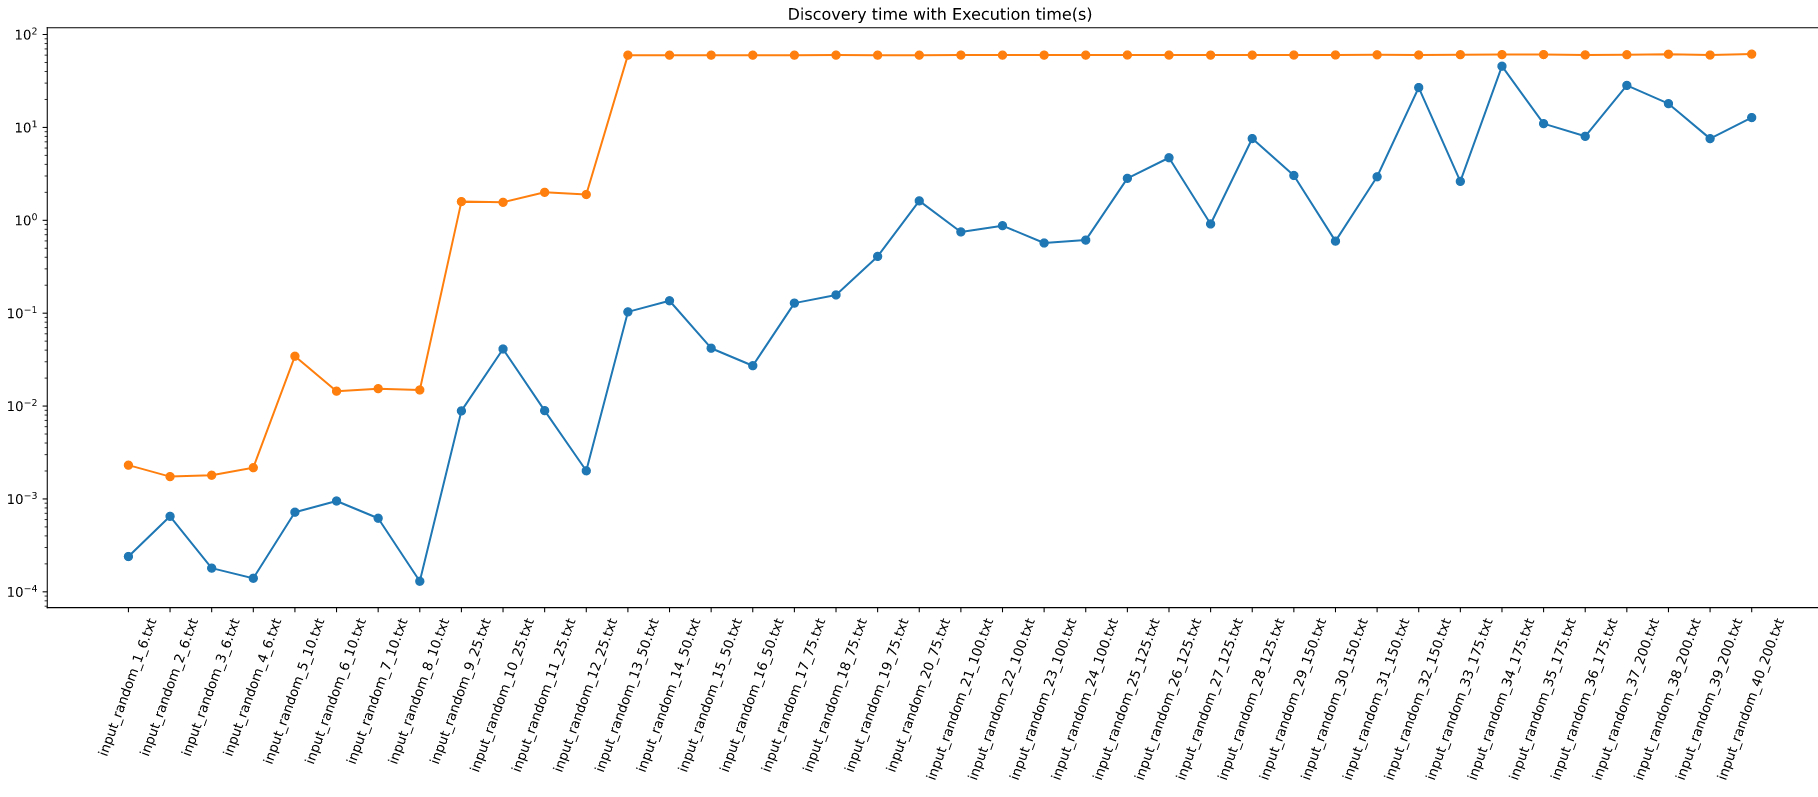
\includegraphics[width=\linewidth]{Img/confronto_time_graph.jpg}
		\caption{Confronto dei Discovery Time rispetto ai tempi totali di esecuzione}
	\end{figure}
\end{center}

\subsection{Grafico di confronto delle percentuali di errore}
\begin{center}
	\begin{figure}[H]
		\centering
		\hspace{-1cm}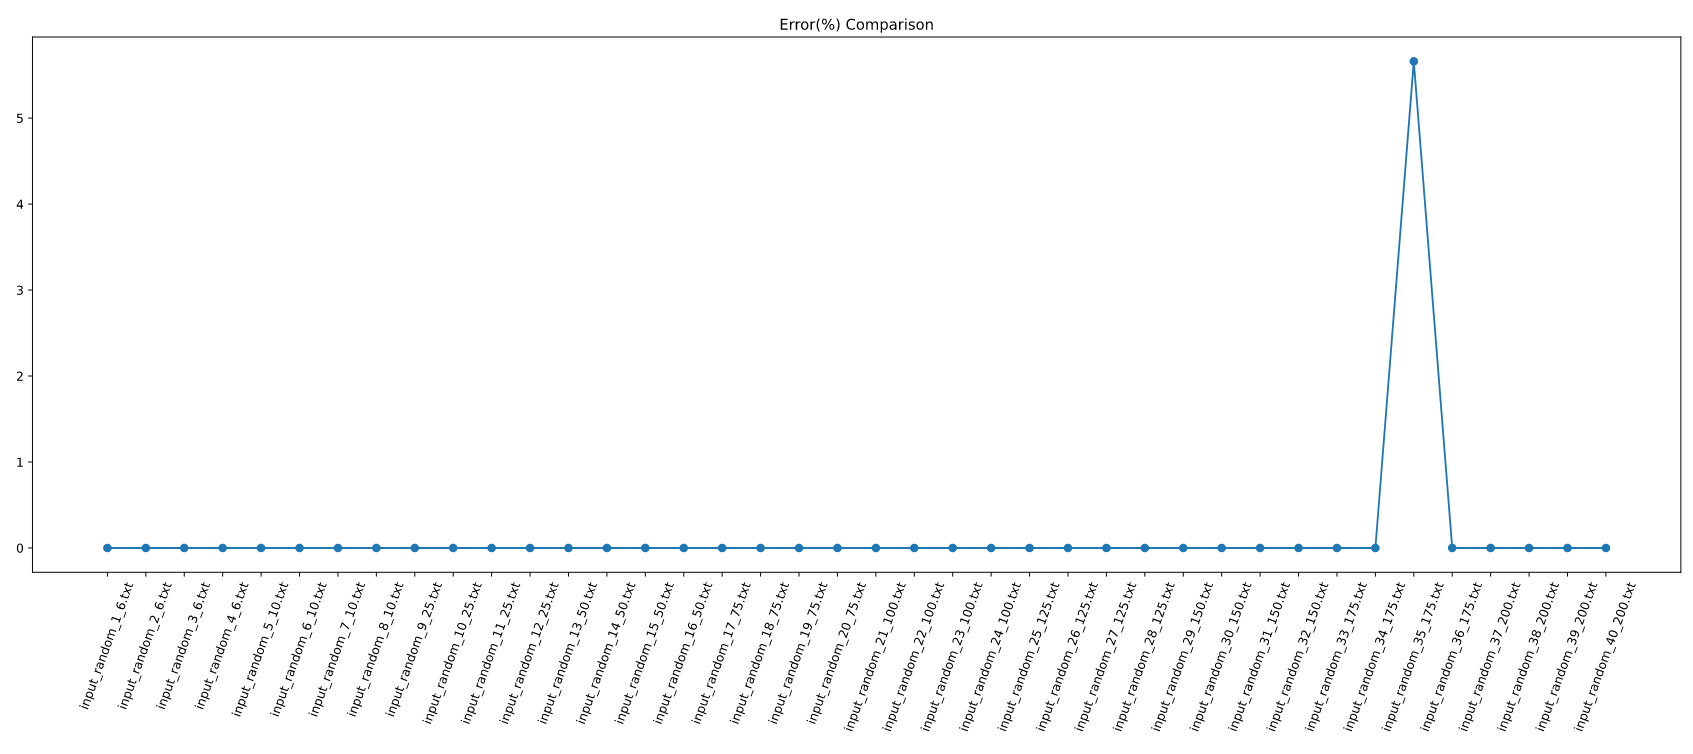
\includegraphics[width=\linewidth]{Img/err_perc_graph.jpg}
		\caption{Confronto delle percentuali di errore}
	\end{figure}
\end{center}

\pagebreak